\chapter{Diagnostics}\label{app:Diagnostics}

The dedicated pedestal experiments, both in I-mode and ELMy H-mode, presented here required an extensive suite of diagnostics to characterize pedestal behavior.  Broadly, these diagnostics may be broken down into three categories:

\begin{description}
 \item[Thomson Scattering] \hfill \\
 Details the edge Thomson scattering diagnostic, from which the high-resolution profile data used for the bulk of this thesis was gathered.
 \item[Fast Diagnostics] \hfill \\
 Details the Electron-Cyclotron Emission (ECE) and $H_\alpha$ line radiation diagnostics used to track sawtooth crashes and ELM events in the plasma edge.
 \item[Fluctuation Diagnostics] \hfill \\
 Details Gas-Puff Imaging (GPI), Reflectometry, and other diagnostics used to characterize the mid-frequency fluctuations found in I-mode pedestals.
\end{description}

\section{Thomson Scattering}\label{sec:app_ts}

Due to the steep gradients in density, temperature, and pressure found in the pedestal, accurate characterization of plasma profiles in this region requires diagnostics capable of very fine spatial resolution.  Measurements based on the Thomson scattering \cite[\S 7]{Hutchinson} of laser light passed through the plasma provides the high-resolution pedestal profiles used in this thesis: Thomson scattering is a near-direct measurement of electron temperature and density, independent of bulk plasma parameters (\ie it is unaffected by the cutoffs or reflections found in other diagnostics, and produces no significant perturbation to the plasma).  Measurement via Thomson scattering produces an effective ``snapshot'' of the plasma parameters at each measurement point, with spatial resolution limited only by collection optics geometry, and time resolution limited by repetition rate on the lasers.  Despite significant technical difficulties -- for example, the high-powered lasers and sensitive collection optics needed to capture the weak scattered light and the necessity for careful calibration of density measurements -- Thomson scattering diagnostics remain a versatile and powerful tool for plasma pedestal measurement, and provided the bulk of the profile data used in this thesis.\nicesectionending

\subsection{Principles of Thomson Scattering}\label{subsec:app_background}

An intuitive picture of the Thomson scattering phenomenon may be obtained by the consideration of a stationary, free charged particle with an EM wave impinging on it.  The particle will be accelerated by the wave (approximately sinusoidally for $E$-field-dominated acceleration at nonrelativistic speeds), causing it to radiate.  Any motion of the particle relative will cause Doppler shifting in the scattered radiation -- motion relative to the incident wave shifts the incident frequency $\omega_i$, at which the particle oscillates, while motion relative to an observer shifts the scattered wave.  This geometry for general positions of the particle and observer is given in \cref{fig:app_ts_geometry}.

\begin{figure}[t]
 \pushtooutside
 \ffigbox[\FBwidth]{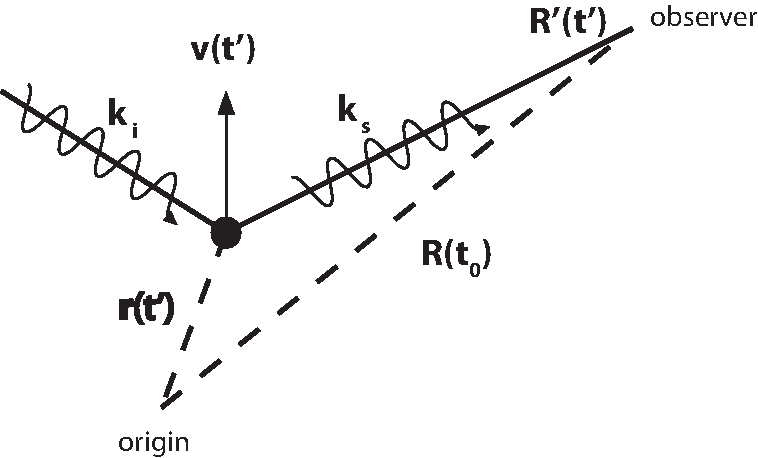
\includegraphics[width=150mm]{graphics/Diagnostics/TS_geometry.pdf}}{\caption{Coordinate system considered for Thomson scattering, with the incident wave of wavenumber $\vec{k}_i$ incident on a particle at $\vec{r}(t')$ for retarded time $t'$.  The scattered wave $\vec{k}_s$ is drawn to an observer at $\vec{R}(t')$.}\label{fig:app_ts_geometry}}
\end{figure}

The scattered electric field from a generally accelerated particle moving at $\vec{\beta} = \vec{v}/c$ is given from the Lienard-Wiechert potentials,

\begin{equation}
 \begin{gathered}
  \vec{E}_s = \frac{q}{4\pi\varepsilon_0} \left[ \frac{1}{\kappa^3 Rc} \hat{s} \times \left( \left(\hat{s} \times \vec{\beta}\right) \times \dot{\beta}\right)\right]_{t'}\\
  \kappa = 1 - \frac{\vec{R}' \cdot \vec{v}}{R'c} = 1 - \hat{s}\cdot\vec{\beta}, \qquad t' = t - \frac{R'}{c}
 \end{gathered}
\end{equation}


\nicesectionending

\subsection{Edge Thomson Scattering on C-Mod}\label{subsec:app_ts_cmod}

\nicesectionending

\section{Fast Diagnostics}\label{sec:app_fast}

\nicesectionending

\section{Fluctuation Diagnostics}\label{sec:app_fluct}

\nicechapterending

\bibliographystyle{../plainurl}
\bibliography{../references}